\chapter{Implementarea aplicației}

Prin parcurgerea acestui capitol, cititorul va avea o imagine de ansamblu asupra modului în care senzorii sunt integrați în aplicație, cum este realizată comunicarea cu serverul și care sunt aspectele legate de programarea și funcționalitatea aplicației mobile. Aceste informații sunt esențiale pentru a înțelege arhitectura și funcționalitatea aplicației în cadrul sistemului smart home propus.

În secțiunea dedicată senzorilor, se vor explora diferite aspecte legate de integrarea lor în aplicație. Această secțiune este alcătuită din subsecțiuni care acoperă următoarele aspecte: module folosite, detalii hardware, programare, prelucrarea datelor, comunicarea cu serverul și controlul prin intermediul telefonului.

În mod similar va decurge și analiza componentei de server care va oferi informații despre dezvoltarea și implementarea \emph{stației de bază}, proxy-ului, rutelor și firewall-ului.

Ultima secțiune, aplicația mobilă, va prezenta detalii despre utilizarea zilnică. Aceasta este deosebit de importantă, deoarece reprezintă interfața principală prin care utilizatorii pot interacționa cu sistemul smart home.

\begin{figure}[h]
	\centering
	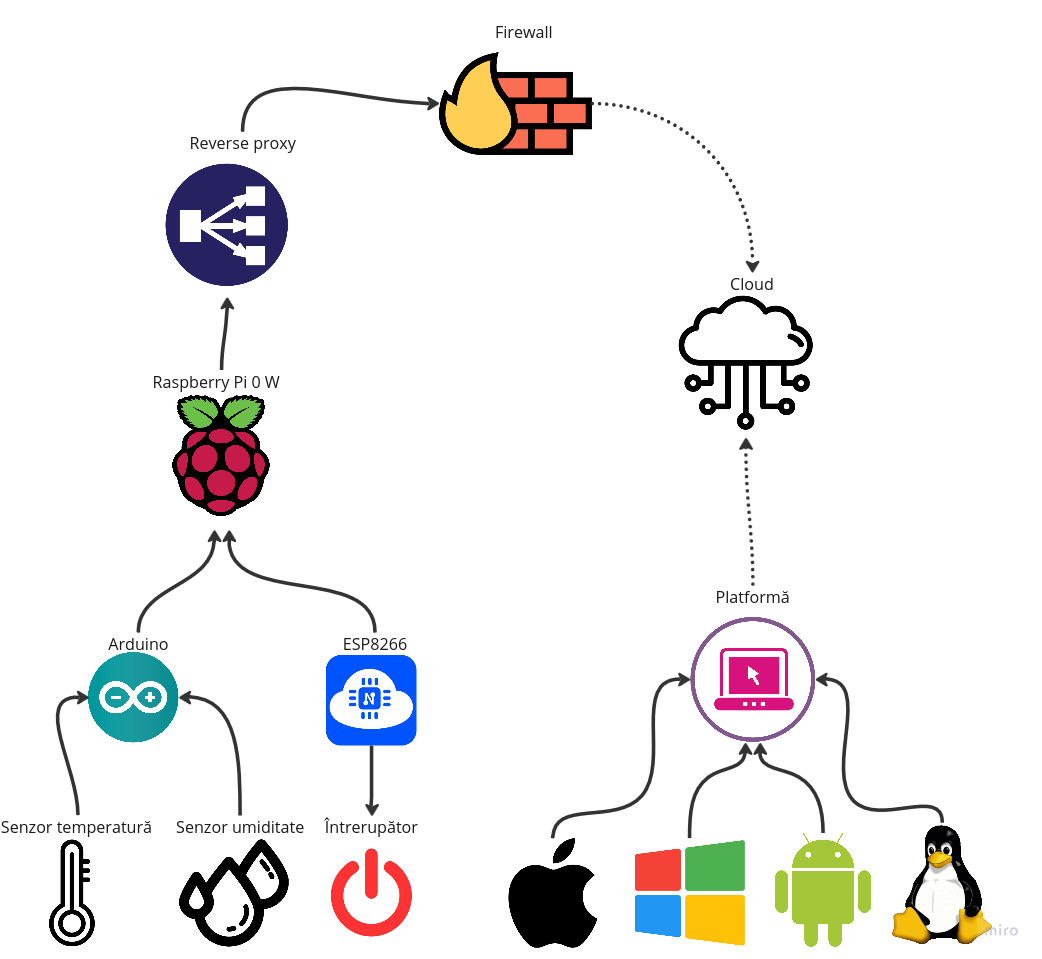
\includegraphics[width=1\textwidth]{arhitectura}
	\caption{Legătura dintre componentele soluției}
	\label{fig:arhitectura}
\end{figure}

\break

\section{Senzori}


\section{Server}

\section{Aplicația mobilă}
